% Chapter Template

\chapter{Related Literature} % Main chapter title

\label{2.} % Change X to a consecutive number; for referencing this chapter elsewhere, use \ref{ChapterX}

%----------------------------------------------------------------------------------------
%	SECTION 1
%----------------------------------------------------------------------------------------

\section{Anomaly or Outlier?}

Generally, there is no agreement on how to distinguish between anomalies and outliers. The following often used citation proves equality of the term outliers and anomalies.\\

\noindent\enquote{\itshape Outliers are also referred to as abnormalities, discordants, deviants, or anomalies in the data mining
	and statistics literature.} - Aggarwal \parencite*{Aggarwal2013}\\

By others, outliers are regarded as corruption in data, while anomalies are abnormal points with a particular pattern. 
In the context of this paper, only the term anomaly is used to refer to such irregular behaviour. It is hereby important to provide a clear definition for the concept of anomaly. This is critical since different meanings of abnormalities necessitate different detection methods. As a result, it is important to identify the key characteristics of anomalies and to use the description to highlight the boundaries. Following, two of the most common definitions of anomalies:\\

\noindent\enquote{\itshape Anomalies are patterns in data that do not conform to a well defined notion of normal behavior.} - Chandola et al. \parencite*{Chandola2009}\\

Ord \parencite*{Ord1996}, defines anomalies as follows:\\

\noindent\enquote{\itshape An observation (or subset of observations) which appears to be inconsistent with the remainder of that set of data.}\\

Anomalies have two major features, according to both of these definitions:

\begin{itemize}
	\item The anomalies' distribution deviates significantly from the data's overall distribution.
	\item Standard data points make up the vast majority of the dataset. The anomalies make up a very small portion of the overall dataset.
\end{itemize}

The development of anomaly detection methods is dependent on these two factors. The second property, in particular, prevents the employment of common classification methods that depend on balanced datasets.

\subsection{Types of Anomalies}
Anomalies come in a variety of shapes and sizes. Anomalies can be divided into three categories:

\begin{enumerate}
	\item \textbf{Point Anomalies} - A point anomaly occurs when a single point deviates dramatically from the rest of the data.
	A point anomaly is, for example, a large credit transaction that differs from other transactions.
	\item \textbf{Collective Anomalies} - Individual points may or may not be anomalous, but a series of points may be. A bank customer, for example, withdraws \$500 from her account per weekday. Although withdrawing \$500 every now and then is common for the consumer, a series of withdrawals is unusual.
	\item \textbf{Contextual Anomalies} - Some points can appear natural in one context but be identified as anomalous in another: In Germany, a daily temperature of 35 degrees Celsius is considered natural in the summer, but the same temperature in the winter is considered unusual.
\end{enumerate}

Knowing ahead of time what kind of anomaly the data might contain helps the data analyst choose the best detection process. Some methods for detecting point anomalies fail to detect collective or contextual anomalies entirely \parencite{Braei2020}.

%\subsection{Time Series Patterns}
%
%There are a few key characteristics of time-series that are briefly described here.
%
%\subsubsection{Level}
%
%The mean of the series is used to determine the time-series standard. When a time-series has a pattern, the level is also said to be changing.
%
%\subsubsection{Trend}
%
%If the mean of a time series does not remain constant over time but increases or decreases, it is said to have a trend. A pattern can be either linear or non-linear in nature. Figure 3 shows a positive trend from 2005 to 2008, and then a downward trend after that.
%
%\begin{figure}[h]
%	\centering
%	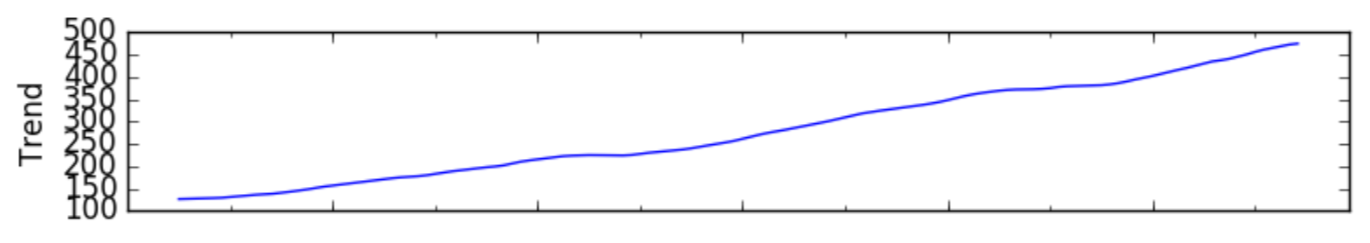
\includegraphics[scale=0.3]{Figures/Trend}
%	\decoRule
%	\caption[Trend]{Trend \parencite{}}
%	\label{fig:Trend}
%	%https://medium.com/swlh/time-series-analysis-7006ea1c3326
%\end{figure}
%
%\subsubsection{Seasonality}
%
%Seasonality refers to the occurrence of variations on a regular basis. Seasonal variables such as the time of year, day of the week, and other similarities influence the time-series, which is why it is called seasonal. As a result, it has a set period of time that is often limited to a year. A seasonal time-series is depicted in Figure 4 \parencite{Braei2020}.
%
%\begin{figure}[h]
%	\centering
%	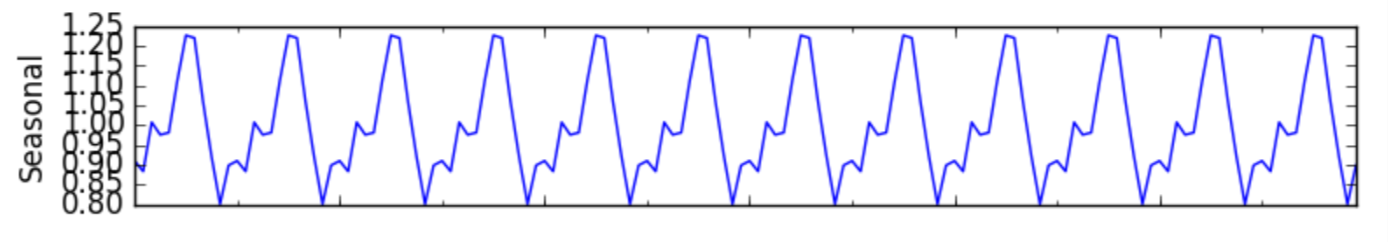
\includegraphics[scale=0.3]{Figures/Seasonal}
%	\decoRule
%	\caption[Seasonality]{Seasonality \parencite{}}
%	\label{fig:Seasonality}
%	%https://medium.com/swlh/time-series-analysis-7006ea1c3326
%\end{figure}
%
%\subsubsection{Noise}
%
%The variability in the observations that the model cannot account for.
%
%\begin{figure}[h]
%	\centering
%	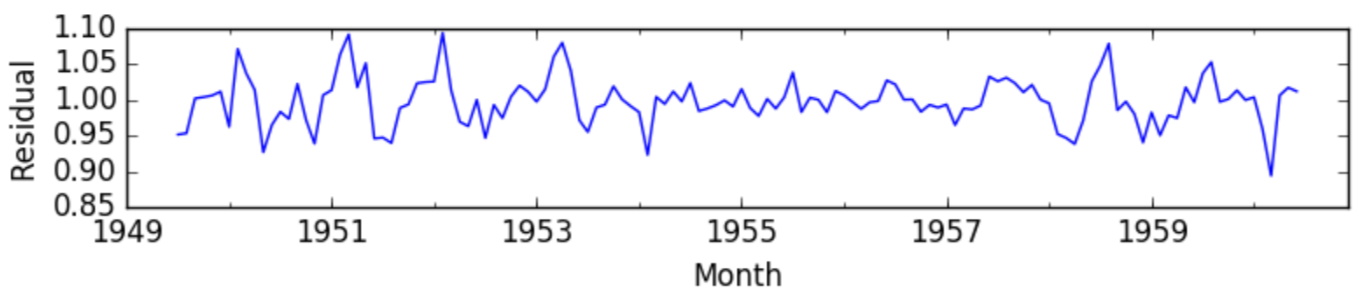
\includegraphics[scale=0.3]{Figures/Residual}
%	\decoRule
%	\caption[Noise]{Noise \parencite{}}
%	\label{fig:Noise}
%	%https://medium.com/swlh/time-series-analysis-7006ea1c3326
%\end{figure}
%
%\subsubsection{Observed}
%
%All the above componenents combined could provide the observed time series shown in Figure . The components may add up to form a model such as: 
%
%\begin{equation}
%	Y =level + trend + seasonality + noise
%\end{equation}
%
%\begin{figure}[h]
%	\centering
%	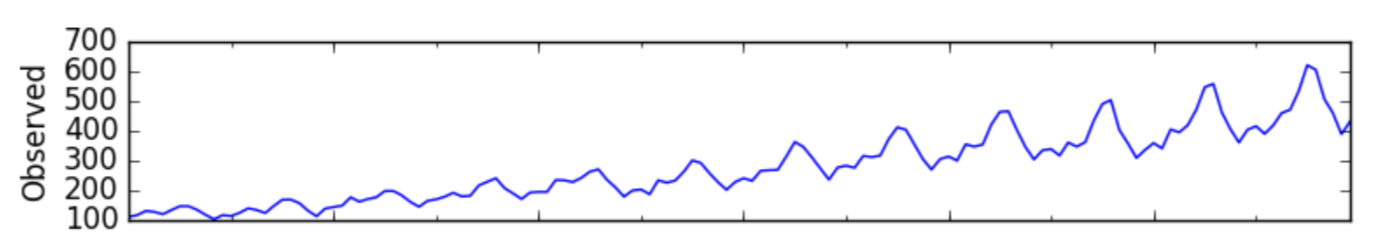
\includegraphics[scale=0.3]{Figures/Observed}
%	\decoRule
%	\caption[Observed]{Observed \parencite{}}
%	\label{fig:Observed}
%	%https://medium.com/swlh/time-series-analysis-7006ea1c3326
%\end{figure}

\section{Anomaly Detection on Univariate Time Series}

First, anomaly detection on univariate time series using deep learning approaches is investigated to gain insight on the used architecture and the overall training and detection process. 

\subsection{LSTM}

Because of their ability to retain long term memory, Long Short Term Memory (LSTM) networks have been shown to be especially useful for learning sequences containing longer term patterns. Malhotra et al. (YEAR) model normal behavior with a predictor and then use the prediction errors to classify abnormal behavior. This is especially useful in real-world anomaly detection scenarios where instances of normal behavior are plentiful but instances of anomalous behavior are rare. For prediction, multiple time steps into the future are forecasted to ensure that the networks capture the temporal structure of the chain. As a result, each point in the series has multiple corresponding expected values made at various points in the past, resulting in multiple error values. The likelihood of normal behavior on the test data is calculated using the probability distribution of the errors produced when predicting on normal data. For this approach Malhotra et al. use a deep LSTM neural network. The proposed network architecture with two hidden layers is successfully applied on different univariate time series such Electrocardiograms (ECG), a valve time series and a power demand dataset. 

In their experiments, Chauhan and Vig (YEAR) used the same approach for different types of anomalies in ECGs such as premature ventricular contractions or atrial premature contractions. 

Especially to mention is the training approach used in both papers. To train the  LSTM based Recurrent Network the data was divided into four sets. a non-anomalous training set, a non-anomalous validation set, a mixture of anomalous and non-anomalous validation set and test set, also consisting of a anomalous and non-anomalous sequences. 

%https://www.elen.ucl.ac.be/Proceedings/esann/esannpdf/es2015-56.pdf


\subsection{CNN}

The use of CNNs for time-series analysis has received interest in recent years. Munir et al. forecast time-series and identify anomalies based on the prediction error using a CNN architecture called deep-learning based anomaly detection method (DeepAnT). DeepAnT uses an architecture that is divided into two modules. The first module is called "Time Series Predictor". The "Time Series Predictor" consists of a CNN. As the name of the module indicates, the CNN is responsible for predicting the future time stamps of a given time series, whereas  the "Anomaly Detector" module is responsible for tagging given data point as anomalous. Figure \ref{fig:CNN} represents the architecture of the CNN-based predictor module. It consists of two convolutional layers, each followed by a max-pooling layer. As the last layer, however, a fully connected layer, where all neurons are connected to all neurons of the previous layer, is used. The last is reponsible for predicting the next time step. The number of output node, hereby, corresponds to the number of predicted time steps. One output node means only the next time step into the future is predicted, whereas three output nodes would imply a sequence of three data points are predicted.     


\begin{figure}[h]
	\centering
	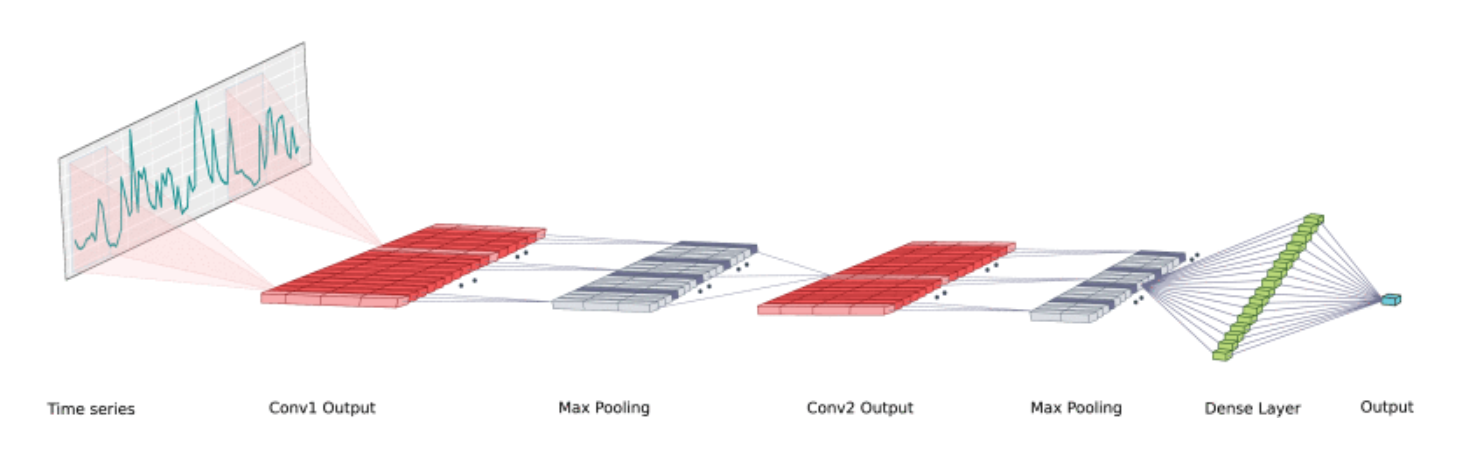
\includegraphics[scale=0.4]{Figures/CNN}
	\decoRule
	\caption[CNN]{CNN \parencite{}}
	\label{fig:CNN}
	%https://ieeexplore.ieee.org/document/8581424?denied=
\end{figure}

Once the next time steps are predicted, the values are then passed to the "Anomaly Detector". The detector module calculates the euclidian distance between the predicted and the actual data point. This measure of discrepancy is used as anomaly score. A high anomaly score indicates a significant anomaly at a given time step. For this module, a threshold based on the time series form must be specified. Most anomaly detection algorithms actually require such a threshold.


\textcolor{red}{ Ioffe and Szegedy suggest another regularization technique called Batch Normalization. Experiments in computer vision showed that Batch Normalization results in a higher learning rate, acts as an alternative for dropout layers and decreases the importance of careful parameter initialization. Therefore, we also implement a CNN architecture using Batch Normalization for univariate anomaly detection to evaluate its performance in anomaly detection.}

\subsection{Comparison}
In an extensive study Braei and Wagner \parencite*{Braei2020} compared 20 different anomaly detection methods. The anomaly detection methods were divided into the three following  categories. 

\begin{itemize}
	\item Statistical Methods
	\item Classical Machine Learning Methods
	\item Deep Learning Based Methods (Neural Networks)
\end{itemize}


\subsubsection{Comparison of AUC}
The methods were applied on data containing point, collective and contextual anomalies. In order to compare the different approaches, AUC-Values \footnote{An ROC curve (receiver operating characteristic curve) is a graph showing the performance of a classification model at all classification thresholds. The AUC measures the entire two-dimensional area underneath the entire ROC curve. See \hyperlink{https://developers.google.com/machine-learning/crash-course/classification/roc-and-auc}{ROC and AUC.}} were used. The results showed that the statistical methods generally performed best on point and collective anomalies while deep learning approaches performed rather poorly. On a dataset that contained contextual anomalies, the situation reflected the exact opposite. Deep learning approaches clearly outperformed statistical methods. It was observed that deep learning approaches kept their ability to generalize while statistical methods overfitted on the data \parencite{Braei2020}.

\subsubsection{Computation Time}
The second parameter that was used to compare the different categories was training and inference time. Inference refers to the time used to classify the test data. Compared to statistical methods and classical machine learning, deep learning approaches once again performed rather poorly regarding training time. Looking at inference time deep learning approches generally perform well, outperforming the other two categories. However, there are huge difference within the deep learning approaches. While CNNs have a very low inference time, and outperform most other algorithms, LSTMs have the highest inference time of all tested algorithms \parencite{Braei2020}.  


%https://arxiv.org/pdf/2004.00433v1.pdf
\section{Anomaly Detection on Multivariate Time Series}

\subsection{LSTM}
%https://nsuworks.nova.edu/cgi/viewcontent.cgi?article=2075&context=gscis_etd

\subsection{CNN}

\subsubsection{Classification of Time Series Data using CNN}
In their research project Zheng et al. (YEAR) tried to beat the state of the art classification algorithm for time series, which is the k-Nearest Neighbor algorithm(k-NN). k-NN has been empirically shown to be extremely difficult to beat. The typical problem of the k-NN algorithm, however, is its computation time. Zheng et al. proposed to use their own developed architecture, which is called Multi-Channel Deep CNN (MC-DCNN). Each channel, hereby represents a CNN with convolutional and pooling layers.
Typically channels in CNN are used to extract features from the different spectra of pictures. A colored picture for example consists of three channels, red, green and blue. Each channel now works as feature extractor on just one color.
This feature of CNN is now used in time series classification. Every channel learns features independently using a single dimension of the multivariate time series as input. Another difference to image classification is that multivariate time series classification uses multiple 1D subsequences rather than 2D image pixels as data. Because CNN only learn features, no classification can be done. In order to classify, a CNN architecture is combined with a Multilayer Perceptron (MLP) that uses fully connected layers. Figure \ref{fig:MC-DCNN} shows the just described architecture. It is important to note that this architecture does not predict the next time steps in the series but instead a given time series is directly classified. The classification is hereby for example used to classify the physical activity depending on the heartrate on is not used for anomaly detection. In order to use the proposed architecture for anomaly detection however, only the output layer has to be changed. 

\begin{figure}[h]
	\centering
	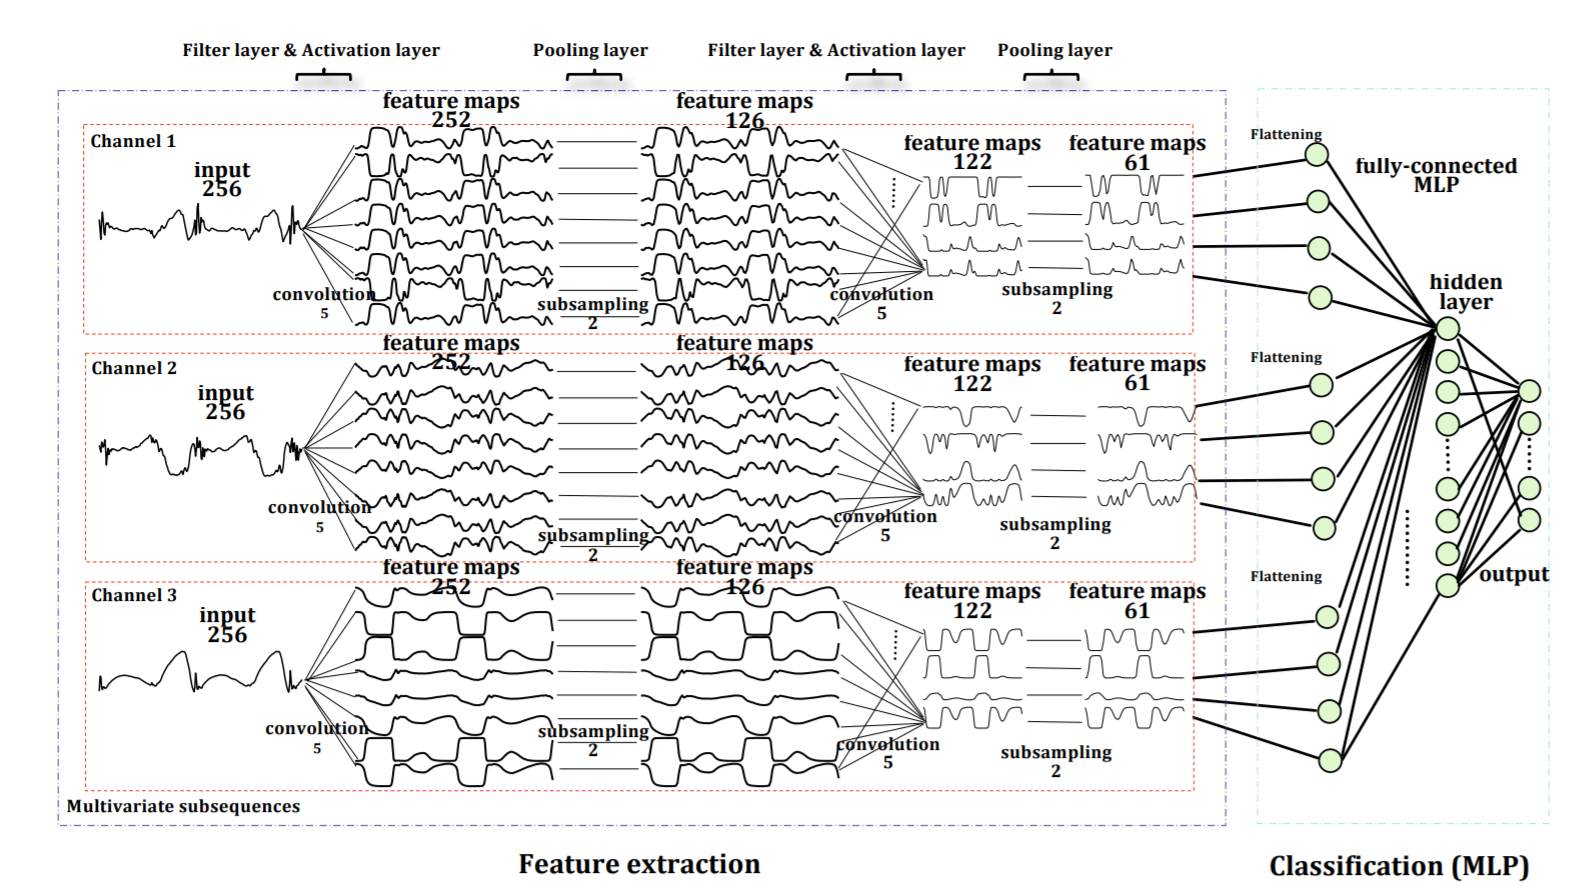
\includegraphics[scale=0.35]{Figures/MC-DCNN}
	\decoRule
	\caption[MC-DCNN]{MC-DCNN \parencite{}}
	\label{fig:MC-DCNN}
	%http://staff.ustc.edu.cn/~cheneh/paper_pdf/2014/Yi-Zheng-WAIM2014.pdf
\end{figure}

Zheng et al. state that the used architecture was superior to the k-NN algorithm regarding accuracy. Further, the experiments shows that deeper architecture are able to learn more robust high-level features. Further, the MC-DCNN architecture performs much faster than the k-NN algorithm, especially when a large dataset is present. 
%http://staff.ustc.edu.cn/~cheneh/paper_pdf/2014/Yi-Zheng-WAIM2014.pdf

\subsubsection{U-Nets for Anomaly Detection}
Wen and Keyes \parencite*{Wen2019} use a special type CNN architecture to detect anomalies. The architecture used is called U-Net. A U-Net consists of so called encoding and decoding layers. The encoding layers work like a standard CNN whereas the decoding layers are used for upsampling. In short, the encoding layers extract the most important features of the time series and decoding layers are using these features to assemble a new time series of the same dimensions as the original one. This encoder-decoder-architecture is often referred to as autoencoder architecture. The main weakness of autoencoders is that in the encoding part through downsampling information is permanently lost. To prevent this information loss, U-Nets introduce so called skip channels also called skip connections. A skip connection, as the name implies, is one that connects an earlier part of the network to a later part of the network and transfers data. The idea is simple: skip channels bring back missing knowledge from some earlier layers so that the network can be properly contextualized. This architecture was proven successful when applied to segmentation of neuronal structures in electron microscopic images in the original paper (Cicek et al., 2016). In order to handle multivariate time series U-Nets also make use multiple channels. Figure \ref{fig:U-Net} shows the architecture of the above described U-Net.

\begin{figure}[h]
	\centering
	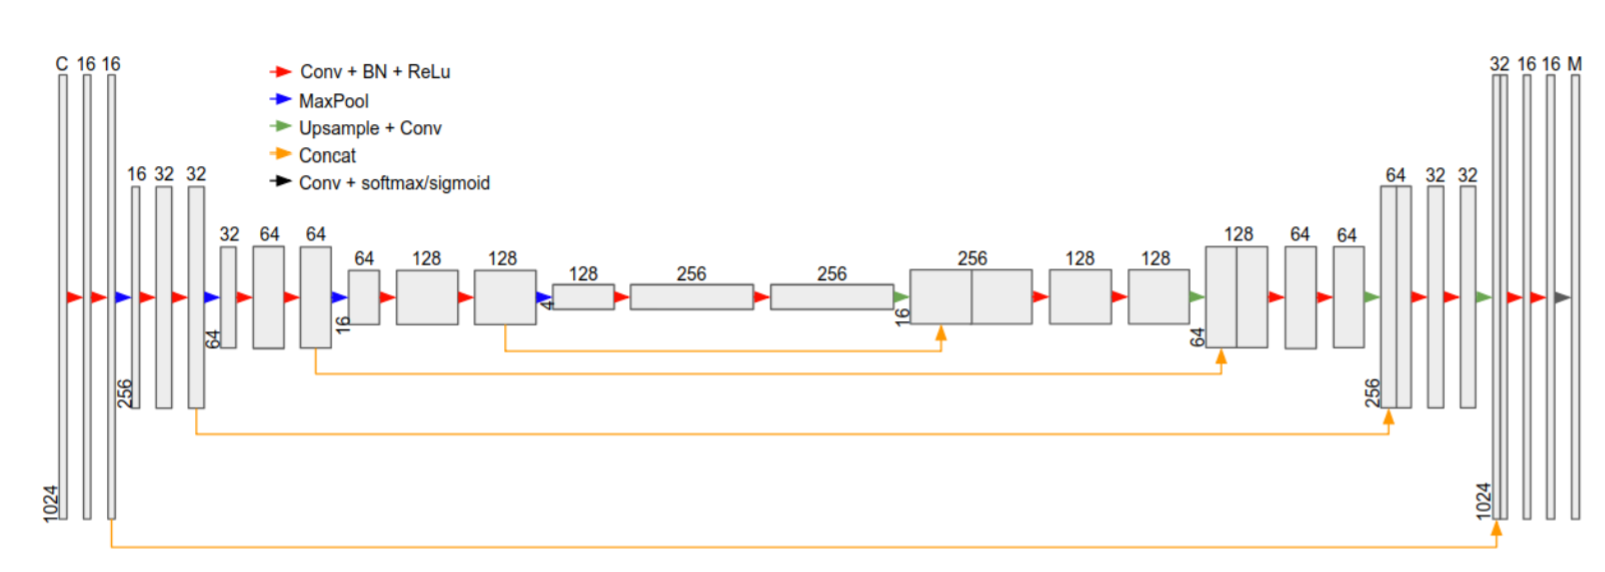
\includegraphics[scale=0.32]{Figures/U-Net}
	\decoRule
	\caption[U-Net]{U-Net \parencite{}}
	\label{fig:U-Net}
\end{figure}

Finally, the model tries to classify what kind of anomaly the multivariate time series contained e.g a seasonal anomaly (contextual) or a point anomaly. Depending on whether the anomaly classes are mutually exclusive or not either a sigmoid or softmax activation is used as last layer activation function.

The proposed U-Net was tested on four scenarios: a univariate task with sufficient data, a multivariate task with sufficient
data, a univariate task with insufficient data and transfer learning, and a multivariate task with insufficient data and transfer
learning. 

For univariate task the dodgers loop sensor data was used. Ihler et al. is the first to introduce this data set2 (2006). It involves a 28-week time series of traffic on a ramp near Dodger Stadium with a 5-minute frequency. The goal is to spot unusual traffic patterns caused by sporting events. Out of 39 events, only three could not be detected. The missing detection were attributed to missing values in the data set. Missing values apparently also were the reason for some false positives.

For the multivariate task the gasoil heating loop data set was used. It contains 48 simulated control sequences for a gasoil plant heating loop that was hacked at one stage. There are 19 variables in all time series. A multivariate U-Net with 19 channels was trained. Out the 18, in the test present attacks, only one was missed. However, also 3 false alarms (false positives) were reported. 

The tasks that included transfer learning are investigated further in section \ref{TransferLearning}.


\section{Parameter Settings for fair comparison}

\section{Transfer Learning} \label{TransferLearning}

\section{Research Gap}
